%\section{Data}
\section{DICOM Data}

To visualize cardiovascular data we first had to search approprite data that exhibit the information we want to visualize.

%\subsection{DICOM}

In the field of medical visualization DICOM is the defacto standard for capturing, annotating and deploying data.
Including meta information and high dynamic range images DICOM is our preferred way to load medical data into our system.

\subsection{Data Acquisition}

To our disappointment we had to find out that it is rather difficult to find appropriate vascular data of the heart.


\subsection{Data Import}

One of the key advantages of DICOM data over simple image stacks is the fact that pixel intensities and radiometric intensities do not need to be the same in a given image stack. So DICOM provides a mapping to use several images together within a homogen radiometric background.


\begin{figure}[h]
	\centering
	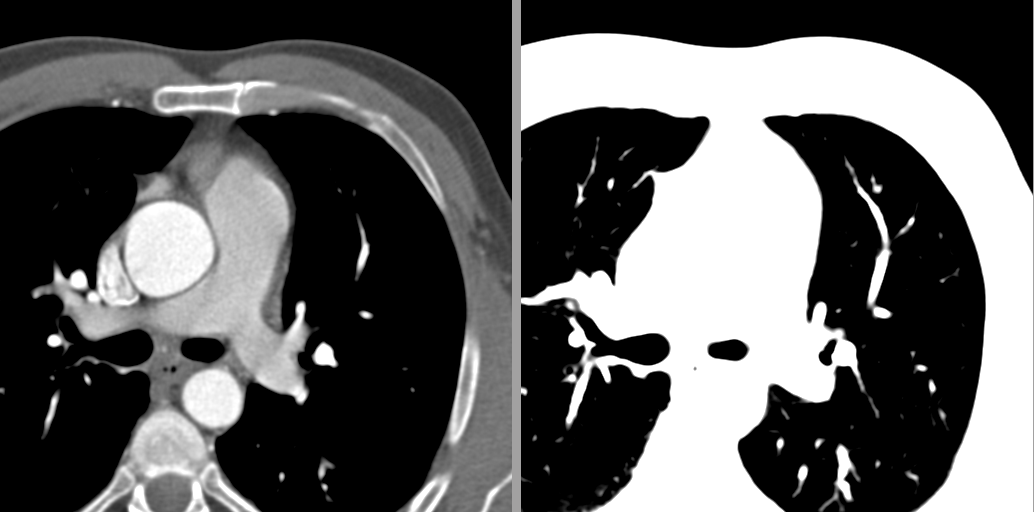
\includegraphics[width=0.45\textwidth]{IM-0001-0019_20.png} \\
	\caption{Stacked images with inhomogenous radiometric space. DIOCM sample data \emph{CARDIX} \cite{gimias_sampledata_2018} aquired from sample data section of the GIMAIS project \cite{gimias_2018} and processed with \emph{dicom2jpeg} from imbera project \cite{imebra_dicom_sdk_2018}.}
	\label{fig:IM-0001-0019_20}
\end{figure}

Simple exports of JPEG data out of DICOM without respecting this relation spills out images with are not homogenous across the stack as seen for instance in figure \ref{fig:IM-0001-0019_20}.


\subsection{Data Conversion}

As it was not possible to find a suitable DICOM reader for our \emph{CARDIX} dataset \cite{gimias_sampledata_2018} for VTK we used an intermediate step via MITK and convert DICOM data with the help of MITK main application to VTK 3D Image (VIK) data readable by VTK.
In this way we could overcome the problems with codecs and intensity differences across the image stack.


